\title{Encoders}
\begin{document}
\section{Encoders}

\begin{frame}{Encoders}
  \begin{definition}
    An \alert{encoder} is a digital logic circuit that accepts $n$ inputs and produces $m$ outputs, where $n>m$.
  \end{definition}
  \begin{itemize}
    \item An encoder is, in some sense, the inverse of a decoder.
    \item The simplest type of encoder is a $2^n$-to-$n$ encoder, or a \alert{binary encoder}.
    \item When put in series after a binary decoder, a binary encoder ``undoes'' the operation of the binary decoder.
  \end{itemize}
\end{frame}

\begin{frame}{Binary encoder logic circuit}
  \begin{columns}
    \begin{column}{5cm}
      \begin{center}
        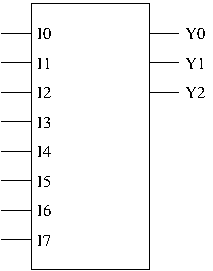
\includegraphics{BinaryEncoderSchematic}
      \end{center}
    \end{column}
    \begin{column}{5cm}
      \begin{center}
        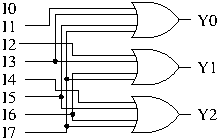
\includegraphics{BinaryEncoderLogic}
      \end{center}
    \end{column}
  \end{columns}
\end{frame}

\section{Priority Encoders}

\begin{frame}{Priority encoders}
  What happens if more than one input is asserted at a time?
  \begin{definition}
    A \alert{priority encoder} ensures that only one input will be used to determine the output.  The inputs are assigned a priority, so that if two inputs are asserted, only one of them ``wins''.
  \end{definition}
  Usually, the most significant input is given the highest priority.
\end{frame}

\section{74x148 Encoder}

\begin{frame}{74x148 priority encoder}
  The 74x148 is a standard priority encoder.\\
  \begin{center}
    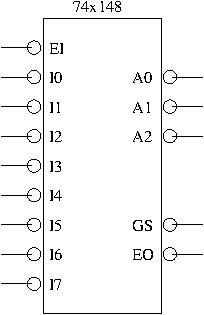
\includegraphics{74x148Schematic}
  \end{center}
  The truth table for this device is shown on page 411 of the text.
\end{frame}

Show the cascading encoders on page 413 of the text.

\end{document}
